

\partabstractfp{进程资源是如何处理的?进程与进程间是怎样的关系?进程死亡后会不会内存泄露?不同生命周期下进程资源的处理方式有什么差异?}
\partabstractrp{注:本章的架构是我根据讲课记录自己的理解划分的,可能与讲课不一致,如有错误欢迎指正。子死父收尸章节应该是第一天讲的,为了保持架构的一致性,把它挪到此处进行处理。}
\partabstractlettrine{从}{出生到死亡,} % the first word of the abstract

\part{进程课第2天}

\chapter{进程出生}
\section{进程出生时资源处理}



\section{进程分裂时的资源变化 -- COW}
父子进程刚诞生时所得到的资源是一样的,那这些资源在何时发生变化,以及变化后有什么影响,这就涉及到了linux的copy-on-write技术,下面通过 具体的实例来说明父子进程的资源变化流程。\\
COW(copy-on-write)技术是进程fork时采用的,涉及到虚拟内存和实际内存的映射关系。采用了COW技术后,进程处理会有一些现象需要重点注意。比如fork之后的父子进程读写同一个全局变量时,一个变量在不同的进程会显示出不同的值。
\subsection{COW 现象代码}
\begin{lstlisting}[language={C}]
#include <stdio.h>
#include <sys/types.h>
#include <unistd.h>
int data = 10;
int child_process()
{
    printf("child process %d, data %d\n", getpid(), data);
    data = 20;
    printf("child process %d, data %d\n", getpid(), data);
    _exit(0);
}
int main(int argc, char * argv[])
{
    int pid;
    pid = fork();
    if(pid == 0){
        child_process();
    }
    else{
        sleep(1);
        printf("parent process %d, data %d", getpid(),data);
        _exit(0);
    }
    return 0;
}
\end{lstlisting}
在正常情况下,程序修改全局变量data,再打印data,会是修改后的值 20,代码中子进程修改全局变量为20后,父进程等待1s,确保子进程已修改完成,但父进程最终打印的结果还是10。
\begin{latexcmd}[label= COW现象]
#运行程序的显示结果如下
child process 9491, data 10
child process 9491, data 20
parent process 9490, data 10
\end{latexcmd}

下面我们具体分析程序背后采用COW的原理和流程。\\
\subsection{COW 实现技术原理}
fork进程前后的内存关系如\ref{linux_fork_mem_compare}所示,
\begin{description}
  \item[\heiti{fork前第1阶段:}] 全局变量data对应数据段内存vir和phy都在数据段,权限为可读可写。
  \item[\heiti{fork后:}] vir和Phy的权限全部变成只读权限,读内存正常,写内存会进入page fault缺页中断。
  \item[\heiti{fork后写内存:}] 写内存后,发生缺页中,Linux会重新申请一个4k内存,将新物理内存指向更改了内存地址的进程vir。同时将老的4k内存拷贝给新的内存,同时将权限改为R+W,这样父子进程的同一个vir虚拟地址就分别对应2个独立的可读可写的物理地址。总之谁先写谁拿到新的物理内存,原内存留给剩下的进程。
\end{description}
\begin{figure}[H]
 \wdfigbox
  {\caption{fork进程前后内存映射关系}\label{linux_fork_mem_compare}}
  {
  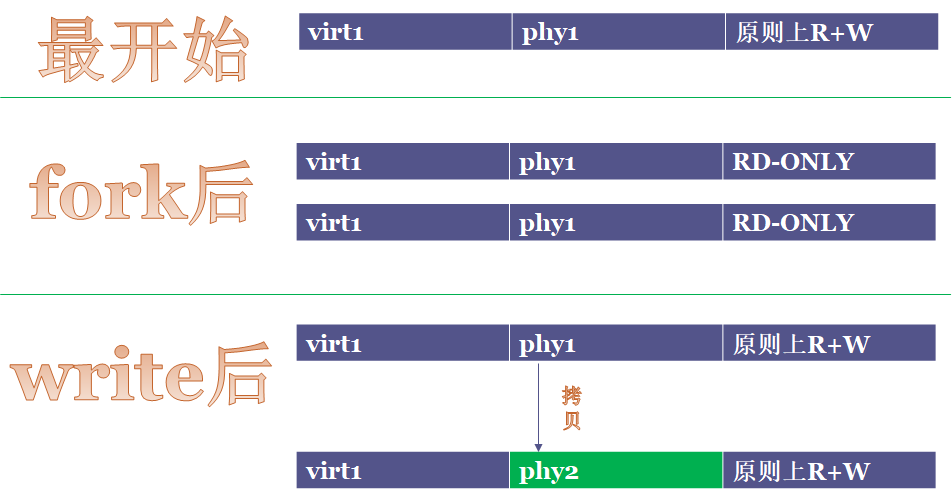
\includegraphics[width=9cm]{./figure/cow_fork_virmem_compare.png}
  \floatfoot{注:第一列为虚拟地址,第二列为物理地址,最后一列对应内存的读写权限 }
  }
\end{figure}
\subsection{无法用COW的情况:VFORK}
COW技术必须借助MMU(内存管理单元)来实现。COW是通过改变虚拟内存和物理内存的映射关系来实现,没有MMU的系统,无法实现虚拟内存和物理内存的映射。也无法调用fork函数,无MMU系统对应调用的是vfork函数,其资源变化对比fork如\ref{vfork_mem}所示:
\begin{figure}[H]
 \wdfigbox
  {\caption{vfork进程内存}\label{vfork_mem}}
  {
  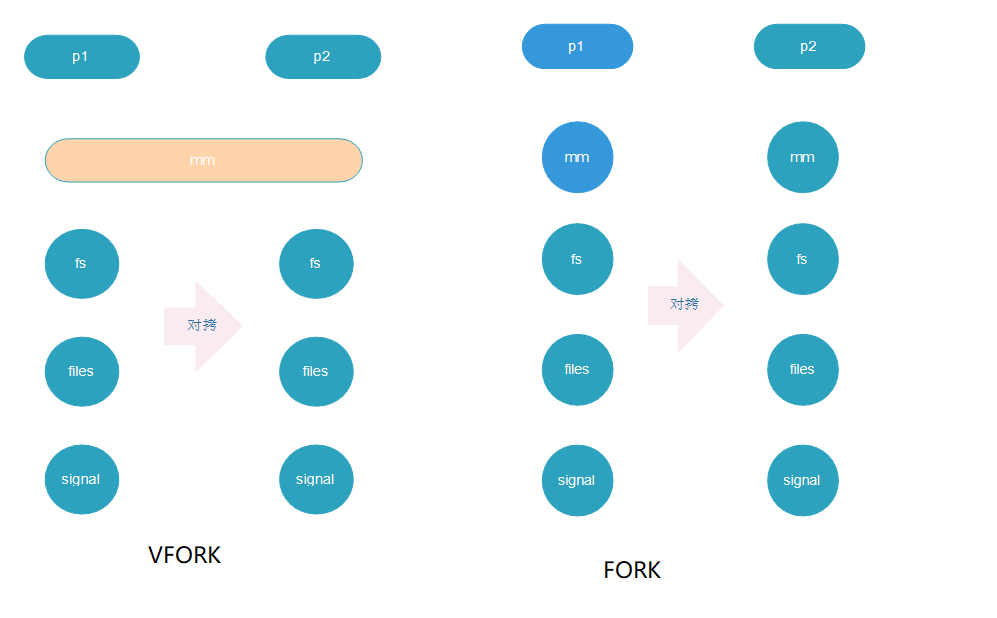
\includegraphics[width=10cm]{./figure/vfork_mem.png}
  \floatfoot{注:mm为同一份,没有进行拷贝  }
  }
\end{figure}
vfork的特点:vfork会阻塞父进程,只有等子进程完全退出后才执行父进程。vfork特性演示视频如下所示:

\begin{tcolorbox}[colback=blue!5,colframe=blue!75!black,title=vfork 视频]
\videoattach{2- vfork.avi}{vfork与COW区别}
\end{tcolorbox}


\section{第1个进程,进程0与进程1}

\chapter{进程运行}
\section{进程睡眠}
\section{进程等待}

\chapter{进程死亡}
\section{子死父收尸}
\section{父死子托孤}
\clearpage
%%% Local Variables:
%%% TeX-master: "main"
%%% End:

